%%%%%%%%%%%%%%%%%%%%%%%%%%%%%
%%%%		INTRODUCTION		%%%%%%%%%
%%%%%%%%%%%%%%%%%%%%%%%%%%%%%

Other examples
Comparison wiith other examples
%\subsubsection{2011 Southwest}
%\subsubsection{2012 India}
%Extremely large

[2] UTCE, “Final Report System Disturbance on 4 November
2006,” Union for the Co-ordination of Transmission of Electricity,
Tech. Rep., 2007.

[3] Interim Report of the Investigation Committee on the 28 September
2003 Blackout in Italy, Union for the Co-ordination of Electricity
Transmission (UCTE), 2003.

[4] Final Report, System Disturbance on 4 November 2006, Union for the
Co-ordination of Transmission of Electricity (UCTE), 2006.

[3] Dam failure triggers huge blackout in Brazil, 2009.

%%%% RELIABILITY

%%%%%%%%%%%%%%%%%%%%%%%%%%%%%%%%%
Hines (2011) Topological Models and Critical slowing down: Two approaches to Power System blackout risk analysis
Disturbances
10 August 1996 Western Interconnect
14 August 2003 North America (1)
4 November 2006 Europe (2)
10 November 2009 South America (3)

Large blackout contribute disproportionaly (4, 5,19)
Risk from vulnerable components (protect components)
risk from operating states close to dynamic instability (avoid these operating states)


%The Value of Reliability in Power Systems: Pricing Operating Reserves (Prada 1999) \cite{prada_1999}

note: One type of output of design problem could be protective relay settings.  when system at nominal condition, it reverts to original protection scheme that protects itself.  when system is precrarious, it goes towards mode that protects entire system for individual component

Corrective switching
 • [Mazi, Wollenberg, Hesse 1986]: Corrective control of power systems flows
 • [Schnyder, Glavitsch 1990]: Security enhancement using an optimal switching power flow  
• [Shao, Vittal 2006]: Corrective switching algorithm for relieving overloads and voltage violations 
Switching to reduce losses 
• [Fliscounakis, Zaoui, et al. 2007]: Topology influence on loss reduction as a mixed integer linear program 
Switching to relieve congestion
• [Granelli, Montagna, et al. 2006]: Optimal network reconfiguration for congestion management by deterministic and genetic algorithms 
Switching to ensure stability 
 • [Perunicic, Ilic, Stankovic 1988]: Short time stabilization of power systems vial line switching 



algorithms to optimize
-variance reduction techniques (common random number)
-derivative free optimization - Torczon et al (generating set search), Conn et al (book), history (Fermi, berman?, other)
-stochastic, mixed integer programing (?????)



cost function of the blackouts
we have estimates of cost few few big blackouts
we say there is a maximum cost for the biggest blackout
fit function to this
use that function for many things


%%%%%%%%%%%%%%%%%%%%%%%%%%%%%%%%%
%%%		MODEL CASCADES		%%%%%%%%%%%%%
%%%%%%%%%%%%%%%%%%%%%%%%%%%%%%%%%

The operator of the power system is able to change branch flows by changing generators dispatch and as last resort load shedding.  At each stage of the cascade, the operator is given a new topology with the loading resulting from the prior stage.  With this, the operator is allowed to change the generator dispatch to minimze cascades.  There are often many constraints on the operators ability to redispatch such as ramping constraints and start/stop times.	

Probalistic
Liao et al (2004) Phase transitions in probability of cascading failures
Mili et al (2004) Risk assessment of catastrophic failures in electric power systems
Chen et al (2005) Cascading dynamics and mitigation assessment in power system disturbances via a hidden failure model
Dobson et al 
(2001)  An initial model for complex dynamics in electric power system blackouts
(2004) Complex dynamics of blackouts in power transmission systems
(2007)Complex systems analysis of series of blackouts: Cascading failures, critical points, and self-organization
 (2011) Exploring complex system aspects of blackout risk and mitigation
Anghel et al (2007) Stochastic model for power grid dynamics
Bienstock (2011)

UNCAT
[21] D. S. Kirschen, D. Jawayeera, D. P. Nedic, and R. N. Allan, “A probabilistic
indicator of system stress,” IEEE Trans. Power Syst., vol. 19,
no. 3, pp. 1650–1657, Aug. 2004.
[22] D. P. Nedic, I. Dobson,D. S.Kirschen, B.A. Carreras, andV. E. Lynch,
“Criticality in a cascading failure blackout model,” Elect. Power Energy
Syst., vol. 28, pp. 627–633, Mar. 2006.
[23] M. Anghel, K. A. Werley, and A. E. Mottor, “Stochastic model for
power grid dynamics,” in Proc.


HIDDEN FAILURES
[11] A. G. Phadke and J. S. Thorp, “Expose hidden failures to prevent cascading
outages,” IEEE Comput. Appl. Power, vol. 9, pp. 20–23, 1996.
[12] S. Tamaronglak, “Analysis of power system disturbances due to relay
hidden failures,” Ph.D. dissertation, Virginia Polytechnic and State
Univ., Blacksburg, VA, 1994.
[13] J. Chen, J. S. Thorp, and I. Dobson, “Cascading dynamics and mitigation
assessment in power system disturbances via a hidden failure
model,” Int. J. Elect. Power Energy Syst., vol. 27, pp. 318–326, May
2005.
11 J. Chen and J. S. Thorp, ‘‘A reliability study of transmission system protection
via a hidden failure DC load flow model,’’ IEEE Fifth International
Conference on Power System Management and Control, 17–19 April
2002, pp. 384–389.


Dobson papers
Two  characteristics, two types

Load based models
Deterministic
Bush (2005) Critical infrastructure protection decission support system project overview
-Critical Infrastructure Protection Decision Support System (CIP/DSS)

Critical Infrastructure Modeling System (CIMS) Idaho National Lab 2005
-What if (Dudenhoeffer et al (2006) - CIMS: a framework for infrastructure interdependency modeling and analysis

Ni et al (2003) Online risk-based security assessment
Zima and Andersson (2004) Wide area monitoring and control as a tool for mitigation of cascading failures


Markov Game Analysis for Attack-Defense of Power Networks Under Possible Misinformation (Ma 2013) \cite{ma_2013}


%%
in some sense, the transition from a unstable, unfeasibil solution to next point is some type of min energy path, or lower point of potential well.  << Lyapanuv functions!!
%%

Vulnerability analysis
Wang (2009) Cascade-based attack vulnerabilities on the US power grid
Bompard (2009) Analysis of structural vulnerabilities in power transmission grids
Arianos (2009) Power grids vulnerabiliites in power transmission grids
Blumsack (2007) a quantitative analysis of the relationship between congestion and reliability in electric power networks


Phase Transition, Lyapunuv
16 C. L. DeMarco, ‘‘A phase transition model for cascading network failure,’’
IEEE Control Syst. Mag. 21, 40–51 ~2001!.


[14] I. Dobson, B. A. Carreras, V. E. Lynch, and D. E. Newman, “An initial
model for complex dynamics in electric power system blackouts,” in
Proc. 34th Hawaii Int. Conf. System Sciences, Maui,HI, Jan. 2001, pp.
710–718.
[15] B. A. Carreras,V. E. Lynch, I. Dobson, andD. E.Newman, “Dynamics,
criticality and self-organization in a model for blackout in power transmission
systems,” in Proc. 35th Hawaii Int. Conf. System Sciences, Big
Island, HI, Jan. 2002.
[16] B. A. Carreras, V. E. Lynch, I. Dobson, and D. E. Newman, “Complex
dynamics of blackouts in power transmission systems,” Chaos, vol. 14,
pp. 643–652, Sep. 2004.
[17] H. Ren, I. Dobson, and B. A. Carreras, “Long-term effect of the n-1
criterion on cascading line outages in an evolving power transmission
grid,” IEEE Trans. Power Syst., vol. 23, no. 3, pp. 1217–1225, Aug.
2008
[18] B. A. Carreras, D. E. Newman, I. Dobson, and N. S. Degala, “Validating
OPA with WECC data,” in Proc. 46th Hawaii Int. Conf. System
Sciences, Wailea, HI, Jan. 2013.

\subsubsection{Notes}

%%%%%%%%%%%%%%%%%%%%%%%%%%%%%%%%%%%%%%%%%%%%%%


Ohm and Kirchoff law not captured well in simple topological models
relationship between physical properties and topo metrics (17,18,10) sometimes correlate to performance

GOAL: Compare vulnerability conclusions from topo measure of vulnerability with more realistic model of power network failure


USed cascading simulation to compare results to some common topological models.  The topo models appear to have erroneous results


Critical slowing down - half of paper, may be interesting to write some up for more depth of generator dynamics


%%%%%%%%%%%%%%%%%%%%%%%%%%%%%%%%%%


  Similar papers have used similar model (4) (19) (24)  (OPA, IMPROVED OPA)


%%%%%%
My hypothesis on how this literature developed, following 2003, large push to understand large scale cascading power failures due to large negative impact on society.  Easiest way to analyze is through the basic topological structure.  The following years saw large amount of papers on topo models to find vulnerabilities.  As these view progressed, realized that topo models had inhearant flaws, exposed by Hines et al. in favor of more realistic flow based models.  During this same time computationale power has increased to point can make use of these more detailed models to find vulnerabilities in this system.  

Perhaps simple paper count of topo models over time from 2000-2012 to show dramatic spike in 2004 and the fall off as the weakness of the models were shown, even though these cascading events keep happening

GOAL: use more realistic model of cascading power failures along with strong computational resources and sold algorithmic development in the computer science and operation research community to solve design problems in the power system arena that address cascading power failure vulnerability


IF Can make connection between LMP and cascades, can use this as motivations for many things
-Electric vehicle, real time pricing
--MAJOR CONCERN FOR FUTURE
--LARGE DELTA ON GRID relative to regular growth patters )  could show contrast to OPA -, it will grow load disportionaly in spots
--THIS WILL MAKE RISK OF CASCADES WORSE
-ECONOMIC MODEL BASED ON VOLATILITY  -- VOLATILITY IS HARMFUL TO SSYSTEM  -- VARIANCE COSTS MONEY, instead we produce at AVERAGE RATE and sell ability to DEVIATE or buy capacity in order to protect UNCERTAINTY IN SYSTEM

-COINCIDENTALLY ?!?!?! the same thing that will put pressure on the grid can help to arbitrage price differentials.  and if large price differtials can make cascades more likely, we WANT THIS BADLY
%%%%%%%%%%%%%%%%%


[28] H. I. Anis, “Probabilistic modeling of power lines magnetic fields,” in
Proc. IEEE Power Engineering


CONTROL
single machine infinite bus voltage problem
Robust and Resilient Control Design for Cyber-Physical Systems with an Application to Power Systems (Zhu 2011) \cite{zhu_2011}




Development of a new algorithm for power flow analysis \cite{mallick_2011}


Power System Analysis and Design Book \cite{glover_2008}


%%%%%%%%%%%%%%%%
DERIVE DC MODEL FROM AC 

Stott (2009) DC power flow revisisted \cite{stott_2009}

Application of Non-linear Programming for Large-Scale AC-DC Power Flow Analysis (Qin 2012) \cite{qin_2012}
Impacts of Topology Control on the ACOPF (Potlurt 2012) \cite{potluri_2012}

Li (2009) decoupled load flow and its feasibility in systems with dynamic topology \cite{li_2009}

Purchala 2005 Usefulness of DC power flow for active power flow analysis 
--ref 36 - incorportation of reactive power flows

--Grijalva 2003 Enhancement of linear ATC calculations by the incorporations of reactive power flows

Overbye 2004 A comparison of the AC and DC power flow models for LMP calculations

prediction of critical load levels for AC optimal power flow dispatch model (bo 2012) \cite{bo_2012}
--polynomial model fitting


Energy Economics
NPV
Time value of money

Levelized Bus-Bar Cost


\subsubsection{Transmission Expansion}
expand capacity or adding lines
$U_e \leftarrow x_e U_e $
%?????$X_e \leftarrow X_e/x_e$ X_e is reactance
where $x$ is the design variable
Transmission Expansion
Security constrained transmission expansion planning: a stochastic multi-objective approach (Akbari 2012) \cite{akbari_2012}
Pozo 2013 A Three-Level Static MILP Model for Generation and Transmission Expansion Planning
AC transmission system planning choosing lines from a discrete set (Gilbertson 2012) \cite{gilbertson_2012}
[32] J. Cui and J. Chen, Design and Building of Overhead Lines. Beijing,
China: China WaterPower Press, 2011.
[29] S. Guo, Basics of Design of Overhead Transmission Lines. Beijing,
China: China Electric Power Press, 2009.



\subsubsection{Vegetation Management}
[24] P. Simpson and R. Van Bossuyt, “Tree—Caused electric outages,” J.
Arboricult., vol. 22, pp. 117–121, May 1996.
[25] D. T. Radmer, P. A. Kuntz, R. D. Christie, S. S. Venkata, and R.
H. Fletcher, “Predicting vegetation-related failure rates for overhead
distribution feeders,” IEEE Trans. Power Del., vol. 17, no. 4, pp.
1170–1175, Oct. 2002.
[26] S. D. Guikema, R. A. Davidson, and H. Liu, “Statistical models of the
effects of tree trimming on power system outages,” IEEE Trans. Power
Del., vol. 21, no. 3, pp. 1549–1557, Jul. 2006.
[27] S. R. Cieslewicz and R. R. Novembri, Utility Vegetation Management
Final Report, CN Utility, LLC, 2004.

\cite{qi_2013}

ELECTRICAL STRUCTURE
Data about topological structure are not sufficient to describe the performance of power networks (24)
connectivity between components
-Sensitivity matrix
--Power transfer distribution factor matricies(41)
-Electrical distances (42) - earliest work
Lagonotte (1989) Structural analysis of the electrical system: Application to secondary voltage control in france
--application to reliability and economic power system problems (43-46)
Lu (1995) A new formulation of generator penalty factors
Hang (2000) A fast voltage security assessment method using adaptive bounding
Zhong (2004) Localized reactive power markets using the concept of voltage control areas
Hines (2008) A centrality measure for electrical networks
Wang (2010) Electrical centrallity measures for electric power grid vulnerability analysis



Analog to diameter  -- the maximum througput of the system to any one node.


MAY BE ABLE TO USE THIS TO FIND AREAS TO IMPROVE THE NETWORK!!!!! positve semi-definate matrix to align search directions

Critical slowing down by \cite{hines_2011} could be informative.


%%%%%%%%%%%%%%%%%%%%%%%%%%%%%%%%%%%%%%%
%%%%%%%%%              STOCHASTIC CASCADE   %%%%%%%%%%%%%%%%%%%%
%%%%%%%%%%%%%%%%%%%%%%%%%%%%%%%%


\chapter{Stochastic Cascade}

\section{Introduction}
A cascading failure is a process in which the failure of a set of components weakens the system and increases the likelihood of future failures of components.  The application to power systems has seen interest due to the large cost to society when one does occur.  It has recently been studied in multiple papers, including a series where Dobson et. al. develop their OPA model.  This models the interaction between the short term force of blackouts and the long term effects of growth and economics for developing the power system.  \\

Assuming the short term force modeled by OPA contains the critical forces determining blackouts, it would be wise to be able to design and upgrade the transmission system to be more robust to these specific forces.  Ignoring environmental causes for faults on power lines, the primary force driving the outage of a single line is the loading.  As the current rises, the temperature of the line will increase which causes effects such as elongation and loss of strength which results in conductor sag and loss of tension \cite{high_temp_std}.  These effects increase the probabilty of line failure.  In the OPA model, this is described as a step function, in which after the line loading is over a certain limit, the probability of failure jumps to $p \in [0, 1]$.  This paper will use a cumulative distribution function to model line failure vs loading, which can reproduce the OPA step function as a special case. \\

The main difficulty in modeling cascading power failures is the decision dependent uncertainty.  The decision operators make determines the power flow on the lines.  The uncertainty in the transition to the next stage is based on the resulting power flow from the operators decision.  In a simulation, this is straightforward as the stages are done sequentialy, so the decisions are made before the outcome of the uncertainty is needed.	\\

The decision dependent uncertainty can also be modeled in the framework of Mixed-Integer Programming (MIP).  MIPs have been used extensively in power systems, helping to solve problems such as unit-commitment \cite{unit_commit} and line switching \cite{line_switch}.  In order to model the availability of lines at a given stage in the cascade, binay variables $ z_t \in \left\{0, 1\right\} $ are used.  These variables along with the failure distribution based on loading are sufficient to model the cascade simulation as a MIP.  \\

The time frame in which cascading failures occur makes it difficult to recognize and react, so it may be best to ensure the system is more robust to cascades before the initial exogenous event occurs.  Using the MIP model of cascades, we develop a planning model which considers multiple contingencies.  A contingency is an initial exogenous event which causes line failures as well as a particular loading.  Assuming a set of contingencies $\Xi$ can be identified through other methods (\cite{vul_region}, \cite{cata_failure})  as the primary risk for initiating a cascading event, this planning model will be able to allocate a budget for transmission expansion optimally in order to reduce the effects of the cascading process.  The process of optimizing a budget over a set of contingencies is known as stochastic programming, and in particular the multiple stages needed to model the cascade process makes it a Multi-Stage Stochastic Program. \\

The main advantage of moving towards the MIP model of cascades is the flexibility it provides.  Having a model which does not have to be simulated in sequational stages gives a more complete mathematical description of the problem.  This description can then be used as a subproblem in a variety of ways.  This paper gives an example of a planning model for transmission expansion, however it could also be used to guide policy decisions such as required operating reserves for given power systems.  However, this flexibility comes at a cost of computational resources.  Stochastic programs are known to be computational intensive for multiple stage problems, which are needed to approximate the effects of cascades due to long chains of events for large blackouts.	\\

The first section of this paper will describe the OPA Model of cascading failures.  This model will then be used to develop the MIP version, which can be shown, with proper parameters, to have the same output as the OPA simulation.  Once the MIP version is known, it can be embedded in a stochastic program.  This will be done through an example of transmission expansion.  Computation results from this program will be shown and conculsions from the results will be drawn.   


\section{OPA Model}

In 2001, Dobson et. al. argued that the power system has self-organized into a dynamic equillabrium where blackouts of all sizes occur \cite{Dobson_2001}.  Their following paper furthers their case for this model representing behavior from the North American power systems.  They note that the average frequency of blackouts in the United states is 13 days and has been the same for 30 years \cite{Carreras_2004}, which appears to represent an equillibrium.  The distribution of blackouts from North American Electrical Reliability Council (NERC) data for the last 15 years follows a power tail curve with an exponent of around $-1.3\pm.2$ \cite{Carreras_2004}.  The model approximates the interaction between the physical system, economic, regulatory, and political responses and blackouts.  The results were consistent with available North American data \cite{Carreras_2004}.   \\

The OPA model begins with an exogenous event, $\xi$, that effects the topology of the grid.  Moments after the outage, the power flows are rerouted through the new topology based on the laws of physics.  In a longer time frame, it is possible for operators to take actions such as load shed and generator redispatch.  The resulting loading on transmission lines is then evaluated with the failure distribution probabilities and after rolling some dice, a transition is made to the next stage.  Either there are no more outages, in which case the cascade is over, or more branch elements are outaged, the topology changes, and the operator is allowed to take recourse.  This process repeats until the system is stable and no outages occur.  

\begin{figure}
\centering
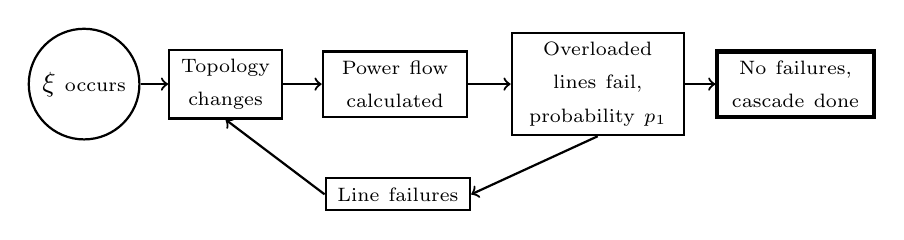
\begin{tikzpicture}
\draw [->,thick] (1,1) node[anchor=east, circle, draw]{$\xi$ \scriptsize occurs}
-- (1.35,1) node(TC)[anchor=west,text width=1.2cm,text centered,  rectangle, draw]{\scriptsize Topology changes};
\draw[->,thick] (TC)
--(3.3,1) node(PF)[anchor=west,text width=1.6cm,text centered, rectangle,draw]{\scriptsize Power flow calculated};
\draw[->,thick] (PF)
--(5.7,1) node(F)[anchor=west,text width=1.95cm, text centered, rectangle, draw]{\scriptsize Overloaded lines fail, probability $p_1$};
\draw[->,thick] (F)
--(8.3,1) node(DN)[anchor=west,text width=1.75cm, text centered,rectangle,draw,line width=1.5pt]{\scriptsize No failures, cascade done};
\draw[->,thick] (F.south)
--(5.2,-.4) node(LF)[anchor=east,text width=1.6cm, text centered, rectangle, draw]{\scriptsize Line failures };
\draw[->,thick] (LF.west)
-- (TC.south);

\end{tikzpicture} 
\caption{OPA simulation of a cascading power failure}
  \label{fig:cascade}
\end{figure}



\subsection{DC Power Flow}

The power flows are determined through the DC power flow model.  This model makes assumptions such as lossless lines, small voltage angle differences, and a flat voltage profile.  It is a common simplifing model which is used routinely in economic analysis of power systems \cite{power_flow}.  The operator of the power system is able to change branch flows by changing generators dispatch and as last resort load shedding.  At each stage of the cascade, the operator is given a new topology with the loading resulting from the prior stage.  With this, the operator is allowed to change the generator dispatch to minimze cascades.  There are often many constraints on the operators ability to redispatch such as ramping constraints and start/stop times.	\\

The following equations represent the necessary constraints on the power flow in this lossless system.  The first equation represents the conservation of energy and the second equation represents Kirchoffs Current Law.

\begin{align}	\displaystyle
\sum_{j \in \cV}{f_{ijn}} &= p_{in} -d_{in} \hspace{20px}   \forall i \in \cV, \forall n \in \cN   \label{pf1}
\\
\theta_{in} - \theta_{jn} &= X_{ij} f_{ijn}			\hspace{20px}	\forall i,j \in \cV, \forall n \in \cN   \label{pf2}
\end{align}


\subsection{Branch Failures}
In order to model a line outage in the DC power flow model, only two changes need to be made the old system.   
\begin{itemize}
\item The power flow on the given branch must be fixed to 0
\item The equation relating phase angles of two connected components removed
\end{itemize}
After making these changes, the resulting model is equivalent to a model of the new topology.  In the simulation it is straight forward to remove constraints.  However, once this model is in the framework of MIPs, some tricks will be needed to convert this logic into mathematical equations.
